% Uses the official CVPR 2026 author-kit style for layout only.
% This independent paper is not a CVPR submission or publication.
\documentclass[10pt,twocolumn,letterpaper]{article}
\usepackage[pagenumbers]{cvpr}
\usepackage{fontspec}
\setmainfont{Liberation Serif}
\setsansfont{Liberation Sans}
\setmonofont{Liberation Mono}[Scale=0.85]
\usepackage{tabularx,array,fvextra,float,microtype}
\definecolor{cvprblue}{rgb}{0.21,0.49,0.74}
\usepackage[breaklinks,colorlinks,allcolors=cvprblue]{hyperref}
\usepackage{newunicodechar}
\newunicodechar{→}{\ensuremath{\rightarrow}}
\newunicodechar{↓}{\ensuremath{\downarrow}}
\newunicodechar{∎}{\ensuremath{\square}}
\providecommand{\tightlist}{\setlength{\itemsep}{0pt}\setlength{\parskip}{0pt}}
\providecommand{\passthrough}[1]{#1}
\newcolumntype{L}{>{\raggedright\arraybackslash}X}
\setlength{\emergencystretch}{2em}
\setcounter{topnumber}{3}
\setcounter{dbltopnumber}{3}
\renewcommand{\topfraction}{0.95}
\renewcommand{\dbltopfraction}{0.95}
\renewcommand{\textfraction}{0.05}
\renewcommand{\floatpagefraction}{0.8}
\title{COVE-3: Budget-Preserving Contour Compilation\\
for Interactive Cube Search}
\author{Rubik's Graph Lab}
\begin{document}
\maketitle
\begin{abstract}

Heuristic search frequently generates successors that are immediately
rejected by a distance bound. We study this overhead in a compact
two-phase Rubik's Cube solver and introduce a project-specific
optimization, budget-preserving contour compilation, within COVE-3. For
each paired phase-2 abstraction, we encode the exact distance and two
successor masks in a 24-bit signature, then replace repeated signatures
with 16-bit dictionary indices. Intersecting the two abstract masks
selects exactly the successors that pass the original heuristic test. A
batched accounting rule charges omitted successors as logical visits,
preserving fixed node budgets and deterministic solution selection. We
prove this equivalence when wall-clock limits do not intervene. On 500
pseudorandom legal states, with five repetitions per configuration, the
compiled solver reduces median latency from 6.19 ms to 2.20 ms and
avoids 79.33\% of recursive calls while returning identical move
sequences and logical visit counts on every case. An ablation retaining
dictionary lookup but disabling selective generation has a median of
7.00 ms. Persistent numeric storage increases from 5.55 MiB to 7.55 MiB,
while dictionary coding uses 31.91\% less storage than a flat compiled
representation. The browser returns its first result using scalar tables
and compiles contours afterward in a worker. The contribution is a
tested optimization of an existing solver; two-phase solving, pattern
databases, and selective generation are established prior work.

\end{abstract}

\hypertarget{introduction}{%
\section{Introduction}\label{introduction}}

A browser solver must balance response latency, memory, solution
quality, and correctness. Exact graph exploration quickly becomes
expensive on the 3×3 Rubik's Cube, whose fixed-frame state space
contains 43,252,003,274,489,856,000 legal positions. Practical two-phase
search offers a useful alternative, but its implementation can still
spend substantial time generating nodes that an existing heuristic
immediately rejects.

Our starting point is the project's scalar two-phase solver, frozen at
its
\href{https://github.com/nahin333/rubikscube/commit/e7023a8d96681c6a4c23a19c4c4ecb5208b910e4}{pre-change
revision}. Its phase-2 DFS applies a move to three coordinates, pushes a
path entry, invokes the recursive routine, and checks the maximum of two
abstract distances. A rejected child has already incurred transition
lookup, path manipulation, and call overhead. In addition, the solver
limits phase-2 visits per subgroup endpoint. Simply removing rejected
calls changes the meaning of that limit and can change which endpoint
succeeds. A faster implementation should make this policy change
explicit or preserve the original behavior.

We develop a compiler for the existing distance tables. A compiled entry
records which moves decrease its distance and which do not increase it.
The two masks suffice because a unit-cost reversible move changes exact
abstract distance by at most one. We intersect filters from both
abstractions and the canonical move-order rule before computing full
child coordinates. Repeated distance-and-mask combinations share a
dictionary entry. We also charge skipped children in their original
order, including visits that trigger a budget guard.

This produces a comparison with a particularly clear quality control:
the old and new solvers return exactly the same move sequence, rather
than merely meeting the same maximum length. Faster execution is
therefore not explained by accepting longer solutions. Initialization
and memory remain separate costs and are measured explicitly.

\hypertarget{contributions}{%
\subsection{Contributions}\label{contributions}}

\begin{enumerate}
\def\labelenumi{\arabic{enumi}.}
\tightlist
\item
  \textbf{A compact compiler for paired phase-2 abstractions.} COVE-3
  combines two contour masks and a distance in a 24-bit signature and
  stores repeated signatures through 16-bit indices. The two product
  tables contain 1,935,360 entries but only 40,609 distinct signatures
  in total.
\item
  \textbf{A budget-preserving selective-generation rule.} We derive
  exact move filters and a batched logical-visit accounting rule,
  proving that fixed-order search retains the scalar solver's outputs
  and count-based stopping behavior when wall-clock guards do not
  intervene.
\item
  \textbf{A controlled implementation study.} We compare the frozen
  scalar solver, a dictionary-only ablation, and the compiled solver on
  500 legal states with repeated measurements, independent sticker
  replay, and exhaustive certificate checks. We report both the latency
  gain and the increased storage cost.
\item
  \textbf{A broader accounting argument and two tested extensions.} We
  extend the count-preservation argument to exact-cost failure
  certificates and deferred sibling charges along single-successor
  chains. Their implementations preserve the tested contract but fail to
  improve latency in a separate evaluation. They remain research
  variants, not enabled application features.
\end{enumerate}

Selective generation itself is established work, including for Rubik's
Cube. Our contribution is this dictionary representation, its
integration with the paired-coordinate solver and visit-budget policy,
and the supporting evaluation. We do not establish that this combination
is the first use of every ingredient in the literature.

\hypertarget{proposed-technical-novelty}{%
\subsection{Proposed technical novelty}\label{proposed-technical-novelty}}

The proposed contribution is a compiler that jointly provides exact
paired-bound successor selection, dictionary sharing of
distance/operator-filter signatures, and scalar-trace equivalence under
fixed count budgets. The specific distinction from the closest
selective-generation precedent \cite{felner2012} is the
budget-preserving transformation and its compact paired-table
representation. Proposition 2 states the preserved contract; the
negative control in Section 6.2 demonstrates what is lost without it.
Our literature review supports this scoped comparison with reviewed
work, while worldwide priority remains unestablished. The
\href{https://github.com/nahin333/rubikscube/blob/main/research/NOVELTY.md}{dated
novelty review} records the scope and overlap explicitly.

\hypertarget{related-work}{%
\section{Related Work}\label{related-work}}

\hypertarget{pattern-databases-and-two-phase-solving}{%
\subsection{Pattern databases and two-phase solving}\label{pattern-databases-and-two-phase-solving}}

Korf combines IDA* with pattern databases to solve Rubik's Cube
optimally \cite{korf1997}. A pattern database stores exact distances in
an abstraction, providing lower bounds for the full problem. Kociemba's
two-phase algorithm first reaches a subgroup and then solves within it
\cite{kociemba_coordinates}; his pruning-table documentation also
describes distance compression using local distance changes
\cite{kociemba_pruning}. COVE-3 follows this decomposition and uses
paired abstractions generated from the application's move geometry.

The directly relevant software baseline is cubejs 1.3.2 \cite{cubejs},
previously used by the application. Its default search target differs
from our scalar solver's first-completion policy. We retain an external
comparison, but use the frozen scalar implementation as the primary
baseline for attribution at identical output quality.

\hypertarget{selective-successor-generation}{%
\subsection{Selective successor generation}\label{selective-successor-generation}}

Felner et al.~introduce enhanced partial expansion and an
iterative-deepening variant that uses operator selection functions to
avoid generating unnecessary children \cite{felner2012}. Their paper
includes Rubik's Cube experiments and discusses pattern-database
operator effects. This is the closest conceptual precedent to our
mask-based generation. Our work specializes the idea to two compact
phase-2 product tables, dictionary-codes the resulting signatures, and
preserves a pre-existing logical visit budget through batched charges.
We claim an implementation improvement with a bounded-policy equivalence
argument, rather than invention of selective generation.

\hypertarget{compression-and-other-objectives}{%
\subsection{Compression and other objectives}\label{compression-and-other-objectives}}

Value compression reduces the set of representable heuristic values
\cite{sturtevant2017}. Our dictionary instead preserves complete
distance-and-operator signatures exactly. Compression itself is prior
work; the object encoded here and its integration with logical-budget
preservation define our proposed contribution.

McAleer et al.~study learned search guidance for cube solving
\cite{mcaleer2018}, while human-oriented methods such as Fridrich's
method optimize recognition and physical execution \cite{fridrich}.
Neither is evaluated as a primary comparator here. Demaine et
al.~analyze generalized cubes \cite{demaine2011}; our optimization
concerns a fixed 3×3 model and does not solve arbitrary-size reduction.
The established 20-move diameter \cite{rokicki_gods_number} concerns
globally optimal paths, whereas our practical solver can return longer
verified sequences.

\hypertarget{transposition-reuse-and-traversal-transformations}{%
\subsection{Transposition reuse and traversal transformations}\label{transposition-reuse-and-traversal-transformations}}

Akagi et al.~analyze correctness and replacement policies for IDA*
transposition tables \cite{akagi2010}. Their work establishes both prior
art for failure reuse and the need to state cache semantics carefully.
Our experimental cache stores an exact logical traversal cost for an
exhausted subtree, rather than a strengthened distance estimate, to
simulate the existing count budget. Replacing recursion with iteration
is also established implementation practice; formal DFS refinement has
been studied by Lammich and Neumann \cite{lammich2015}. Neither caching
nor iterative traversal is claimed as our invention. The additional
research question is preservation of this solver's count-based
observations under these transformations.

\hypertarget{problem-formulation}{%
\section{Problem Formulation}\label{problem-formulation}}

Let \(s_0\) be a legal 3×3 state, \(s_\star\) the solved state, and
\(T\) the move transition function. A solution is a sequence
\(\pi=(a_1,\ldots,a_L)\) with \(T(s_0,\pi)=s_\star\). We use the
half-turn metric: each outer-face quarter turn, inverse quarter turn, or
half turn costs one.

A cubie state contains corner and edge permutations \(p_c,p_e\) and
orientations \(o_c,o_e\). Legal states satisfy

\[
\begin{gathered}
\sum_{i=0}^{7}o_{c,i}\equiv0\pmod3,\qquad
\sum_{i=0}^{11}o_{e,i}\equiv0\pmod2,\\
\operatorname{parity}(p_c)=\operatorname{parity}(p_e).
\end{gathered}
\tag{1}
\]

The two-phase solver first reaches
\(H=\langle U,D,R^2,L^2,F^2,B^2\rangle\). Phase 1 uses corner
orientation, edge orientation, and middle-slice membership coordinates
of sizes 2187, 2048, and 495. Phase 2 preserves \(H\) with ten moves and
uses corner permutation \(c\), non-slice-edge permutation \(e\), and
slice-edge permutation \(q\), with sizes 40320, 40320, and 24. Its lower
bound is

\[
h_2(c,e,q)=\max\{D_C(c,q),D_E(e,q)\},
\tag{2}
\]

where \(D_C,D_E\) are exact distances in the two product abstractions.
Abstract paths are projections of full paths, so this maximum is
admissible. Our optimization preserves this bound and its accepted
successors.

We distinguish a \textbf{logical visit}, charged by the scalar routine
even when immediately pruned, from a \textbf{generated visit}, where the
optimized routine actually constructs child coordinates and enters DFS.
Visits count search-tree occurrences, including iterative-deepening
repeats; they are not distinct cube states.

\hypertarget{methodology}{%
\section{Methodology}\label{methodology}}

\hypertarget{system-and-baseline-policy}{%
\subsection{System and baseline policy}\label{system-and-baseline-policy}}

COVE-3 denotes Compact Output-Verified Exploration for 3×3. The
application accepts typed turns or manually corrected photo-derived
stickers, validates the symbolic cube, runs search in a worker, and
replays returned moves on the sticker model. The photo interface is not
a learned recognition model.

\begin{figure*}[t]
\centering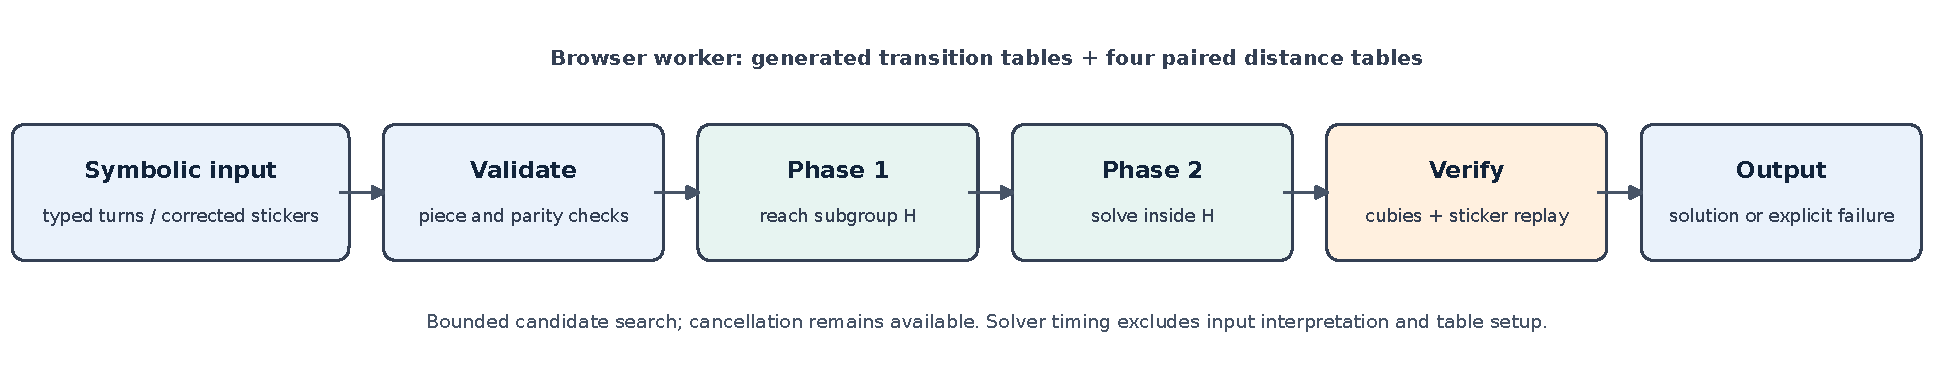
\includegraphics[width=\textwidth]{figures/system-pipeline.pdf}
\caption{Browser execution. The first scalar result is posted before contour compilation; later solves use compiled tables. Photo-derived stickers require manual correction and are not an autonomous vision benchmark.}
\label{fig:system-pipeline}
\end{figure*}

The frozen baseline limits phase 1 to depth 12 and each phase-2 attempt
to depth 18. A subgroup endpoint receives 250,000 phase-2 logical visits
across its iterative-deepening attempts. The global limit is 20 million
logical visits. A guard can count the extra visit that triggers it. Time
is checked every 2048 logical visits, with a 30-second search deadline
and a separate 45-second browser-worker watchdog. The first completion
is accepted after cubie and sticker verification. Consecutive same-face
moves are excluded, and commuting opposite faces use a canonical order.

\hypertarget{exact-contour-filters}{%
\subsection{Exact contour filters}\label{exact-contour-filters}}

For either abstraction, let \(D(a)\) be its exact goal distance and
\(\delta(a,m)\) its successor under phase-2 move \(m\). Define

\[
\begin{aligned}
M_-(a)&=\{m:D(\delta(a,m))=D(a)-1\},\\
M_0(a)&=\{m:D(\delta(a,m))\le D(a)\}.
\end{aligned}
\tag{3}
\]

These sets are ten-bit integers. At remaining depth \(r\ge D(a)\), the
moves that can pass the next scalar heuristic check are

\[
F(a,r)=
\begin{cases}
M_-(a),&r=D(a),\\
M_0(a),&r=D(a)+1,\\
\mathcal A_2,&r\ge D(a)+2.
\end{cases}
\tag{4}
\]

Let \(A_\ell\) encode the canonical moves allowed after face \(\ell\).
The full admissible successor mask is
\(A_\ell\cap F((c,q),r)\cap F((e,q),r)\). Set bits are processed in the
original increasing move-index order.

\textbf{Proposition 1 --- Exact successor filtering.} For an admitted
phase-2 node, the compiled mask contains a canonical move if and only if
the scalar child's heuristic is at most \(r-1\).

\emph{Proof.} Because each phase-2 move has an inverse and unit cost,
applying a move changes exact abstract distance by at most one. If
\(r=D(a)\), only a distance decrease can reach \(r-1\). If \(r=D(a)+1\),
a non-increase suffices. If \(r\ge D(a)+2\), even a one-step increase is
at most \(r-1\). These are exactly Eq. (4). Intersecting both
abstractions implements the maximum in Eq. (2), and intersecting
\(A_\ell\) imposes the same canonical rule as the scalar loop. ∎

\hypertarget{dictionary-representation}{%
\subsection{Dictionary representation}\label{dictionary-representation}}

For every paired abstract state, the compiler forms

\[
\sigma(a)=\bigl(D(a)\ll20\bigr)
\mathbin{|}\bigl(M_0(a)\ll10\bigr)
\mathbin{|}M_-(a).
\tag{5}
\]

The measured maximum distances are 14 and 12, so four distance bits and
two ten-bit masks fit in 24 bits. Compilation checks the distance bound,
the one-step distance-change property, and dictionary capacity. It
interns equal signatures and stores a 16-bit index per abstract state;
signatures occupy 32-bit dictionary entries. Corner/slice and edge/slice
tables use 5806 and 34,803 signatures respectively. The extra lookup
trades a small amount of indirection for fewer signature bytes.

The uncompiled phase-2 tables contain \(D_2=2(40320\cdot24)=1,935,360\)
byte distances. Let \(D_1=2187\cdot495+2048\cdot495=2,096,325\) and
\(M_T=1,783,560\) be phase-1 distance bytes and all transition bytes.
With \(U=40,609\) signatures,

\[
\begin{aligned}
M_{\rm scalar}&=M_T+D_1+D_2\\
&=5,815,245\ \text{bytes},\\
M_{\rm dict}&=M_T+D_1+2D_2+4U\\
&=7,913,041\ \text{bytes},\\
M_{\rm flat}&=M_T+D_1+4D_2\\
&=11,621,325\ \text{bytes}.
\end{aligned}
\tag{6}
\]

The flat value is the calculated footprint of storing one 32-bit
signature at every paired index, not a measured flat-solver latency. The
dictionary saves 31.91\% relative to that representation but increases
persistent storage by 36.07\% relative to byte distances. None of these
figures measures peak JavaScript heap, temporary BFS queues, hash-map
overhead, or renderer memory.

\hypertarget{preserving-the-search-budget}{%
\subsection{Preserving the search budget}\label{preserving-the-search-budget}}

Skipping rejected children without accounting would allow the optimized
search more admitted work under the same nominal node cap. Instead,
before each selected move we count canonical rejected moves preceding it
and charge their visits in a batch. We charge remaining rejected
siblings afterward. Charging stops at the earliest endpoint or global
guard and retains each periodic time/progress checkpoint. A rejected
child needs no path mutation or coordinate construction.

\begin{figure}[t]
\hrule\vspace{5pt}
\textbf{Algorithm 1.} Budget-preserving phase-2 expansion
\vspace{4pt}
\begin{Verbatim}[fontsize=\footnotesize,breaklines=true,breakanywhere=true]
Input: phase-2 coordinates (c,e,q), depth r, last face l
charge one generated visit; enforce guards
if h2(c,e,q) > r: return failure
if r = 0: return whether coordinates are solved
A = canonical move mask after l
M = A & cornerContour(c,q,r) & edgeContour(e,q,r)
for each set bit m of M, in original move order:
  charge uncharged rejected moves of A preceding m
  stop immediately if a budget is exhausted
  construct child coordinates and push m
  if recursive search succeeds: return success
  pop m; stop if a budget is exhausted
charge remaining rejected moves of A
return failure
\end{Verbatim}
\vspace{3pt}\hrule
\end{figure}

\textbf{Proposition 2 --- Count-budget trace equivalence.} For identical
tables, input, depth limits, move order, and logical node budgets,
scalar and compiled search return the same move sequence, phase split,
and logical count, or fail at the same count-based guard, provided a
wall-clock guard does not intervene.

\emph{Proof.} By Proposition 1, every omitted child would return
immediately after its logical-visit and endpoint checks. Replace each
such call with one charge, preserving sibling order. The remaining
recursive calls have identical coordinates and path prefixes. Induction
over DFS calls preserves the successful path or exhaustion outcome.
Truncating each charge batch at the first guard preserves endpoint
abandonment and global failure. Iterative-deepening iterations and
phase-1 endpoints therefore remain identical. Periodic count checkpoints
are retained even inside a batch. Real wall-clock outcomes need not
match because execution time changes. ∎

\hypertarget{complexity-comparison}{%
\subsection{Complexity comparison}\label{complexity-comparison}}

Let \(b_1\le18\), \(b_2=10\), and \(d_1\le12,d_2\le18\) bound branching
and depth. Write \(R_j(d)=\sum_{k=0}^{d}\sum_{i=0}^{k}b_j^i\), a
conservative \(O((d+1)b_j^d)\) iterative-deepening bound. If \(C\)
phase-1 endpoints are attempted, the scalar logical-visit bound is
\(R_1(d_1)+C R_2(d_2)\) before resource limits, and at most \(G+1\)
visits under a global budget \(G\). Compilation preserves this bound; it
reduces generated work rather than enlarging the logical allowance.

Let \(k_v\le b_2\) be the number of successors passing both abstract
tests at expanded phase-2 node \(v\). Scalar expansion constructs up to
\(b_2\) children. Compiled expansion uses constant-time mask operations
and iterates \(k_v\) selected bits, with constant-cost charges between
them for the fixed ten-move domain. It therefore costs \(O(1+k_v)\) per
admitted expansion instead of \(O(b_2)\). If every move passes, the
orders agree. Both algorithms remain exponential in depth in the worst
case.

Let \(S_1=2187+2048+495\) and \(S_2=40320+40320+24\). Scalar
preprocessing performs \(O(18(S_1+D_1)+10(S_2+D_2))\) coordinate
transitions and BFS edge checks. Compilation adds \(O(10D_2)\) work
under the usual expected constant-time hash-table assumption for
signature interning. With \(M_T\) transition bytes excluded, both
representations use \(O(D_1+D_2)\) persistent space because
\(U\le D_2\). Their byte constants differ as in Eq. (6). Search
stack/path space remains \(O(d_1+d_2)\), endpoint conversion costs
\(O(d_1)\) per attempt, and sticker replay costs \(O(54L)\) for a
returned path of length \(L\).

\begin{table*}[t]
\caption{Complexity relative to the actual scalar baseline. Both methods retain exponential worst-case search; compiled expansion avoids constructing rejected children.}
\centering\small
\begin{tabularx}{\textwidth}{@{}p{0.20\textwidth}LLp{0.22\textwidth}@{}}
\toprule
Operation & Scalar baseline & Compiled COVE-3 & Interpretation \\
\midrule
One admitted phase-2 expansion & \(O(b)\) & \(O(1+k)\) & Avoids rejected child construction \\
Extra contour preprocessing & None & \(O(bD_2)\) expected & Paid before compiled solves \\
Persistent abstract storage & \(O(D_1+D_2)\) & \(O(D_1+D_2+U)\) & Same order, larger measured constant \\
Stack/path storage & \(O(d_1+d_2)\) & \(O(d_1+d_2)\) & Same order \\
Worst-case unrestricted search & Exponential in depth & Exponential in depth & No asymptotic superiority claimed \\
\bottomrule
\end{tabularx}
\end{table*}

For a fixed 3×3 cube the coordinate dimensions are constants. These
parameterized bounds describe implementation costs and do not imply a
generalized-cube complexity result.

\hypertarget{exact-cost-failure-certificates}{%
\subsection{Exact-cost failure certificates}\label{exact-cost-failure-certificates}}

Consider an exhausted phase-2 subtree identified by
\(x=(c,e,q,r,\ell)\), where \(r\) is remaining depth and \(\ell\) is the
last face. The last face is essential because it determines canonical
move exclusions. Let \(w(x)\) be its complete scalar logical visit
count, including its root. Store \((x,w)\) only after failure without an
endpoint cutoff. A success, interrupted traversal, or budget-truncated
failure is not a reusable failure certificate.

After the root visit has been charged normally, a matching certificate
can replace the remaining traversal only if

\[
w(x)-1\le\min\{B-n_E,\ G-n_G\},
\tag{7}
\]

where \(B,G\) are endpoint and global caps and \(n_E,n_G\) their current
counts. Otherwise the original traversal runs, preserving the precise
cutoff boundary. A direct-mapped table stores full numeric keys, so a
hash collision causes replacement or a miss, never false equality. The
prototype has \(2^{16}\) slots, with a Float64 key and Uint32 cost per
slot: 786,432 additional bytes (0.75 MiB) allocated per solve. It probes
only admitted states with remaining depth 3 through 8.

\textbf{Proposition 3 (failure-certificate replay).} In this fixed-order
search, replacing an exhausted subtree satisfying (7) by its exact
remaining logical count preserves returned moves, count-based cutoffs,
and count-indexed progress notifications, provided the original periodic
checkpoints are retained and no wall-clock limit intervenes.

\textbf{Proof.} The phase-2 coordinates determine the full subgroup
state; remaining depth and last face determine its finite, ordered
search tree. There is no additional ancestor-dependent cycle exclusion.
Exhaustion establishes that the subtree returns false, so it cannot
contribute a selected solution. Equation (7) ensures the replaced
segment cannot cross a count cutoff. Charging its exact remaining
length, with every periodic checkpoint, reaches the same observable
counter state as the explicit traversal. Induction over such
substitutions gives the result, including when a stored cost was
measured with earlier valid substitutions. Full-key equality and storage
only after exhaustion make replacement policy irrelevant to soundness.
Elapsed timestamps and real-time timeout outcomes are outside the claim.

For a certificate of cost \(w\), replay costs \(O(1+w/J)\) rather than
explicit traversal, where \(J=2048\) is the mandatory checkpoint
interval. Cache initialization costs \(O(K)\) for \(K\) slots, lookup is
\(O(1)\) for the fixed direct-mapped scheme, and storage is \(O(K)\).
Misses, collisions, and lookup overhead remain; exponential worst-case
search is unchanged. Fewer generated visits do not imply lower measured
latency.

\hypertarget{deferred-sibling-charges-along-single-successor-chains}{%
\subsection{Deferred sibling charges along single-successor chains}\label{deferred-sibling-charges-along-single-successor-chains}}

When exactly one child survives the contour masks, all other permitted
children are known to fail immediately. Charge rejected siblings before
that child immediately, then descend iteratively. Rejected siblings
after it must be charged only if the child fails. Their counts
accumulate as a deferred scalar debt along the chain; a successful
descendant discards that debt, while a failed descendant charges it with
the existing capped checkpoint routine before returning.

The invariant is that accumulated debt counts only pending, immediately
rejected siblings on the active chain. On failure their charges are
contiguous after inner subtrees finish, so combining them preserves
count-indexed observations; on success the original DFS never visits
them. Intermediate cutoff handling truncates debt at the original guard.
Thus the transformation preserves the same contract as Proposition 2. It
changes recursion into iteration without skipping generated states,
strengthening the distinction between call counts and search work. It
adds \(O(1)\) debt storage per active recursive frame and retains
\(O(d_2)\) path/stack space and exponential worst-case work. The
experiment records removed recursive calls separately from generated
visits.

\hypertarget{experimental-setup}{%
\section{Experimental Setup}\label{experimental-setup}}

\hypertarget{questions-and-configurations}{%
\subsection{Questions and configurations}\label{questions-and-configurations}}

We ask whether compilation improves latency at identical output quality
(RQ1), whether selective generation explains the improvement (RQ2), and
how storage and application behavior change (RQ3). The primary
configurations are:

\begin{itemize}
\tightlist
\item
  \textbf{Original scalar:} the actual frozen pre-change solver, loaded
  from the pinned revision in the same JavaScript realm as the
  candidate.
\item
  \textbf{Dictionary + scalar:} the current solver with dictionary
  lookups and visit bookkeeping, but ordinary recursive child
  generation. This ablates the mask-based generator.
\item
  \textbf{Compiled COVE-3:} dictionary lookup, exact mask intersection,
  and batched logical charging.
\end{itemize}

All configurations retain the same distance bounds, move order, endpoint
cap, global cap, and phase depth limits. We assert equality of complete
move sequences, phase splits, and logical visit counts rather than
comparing average lengths alone. Each returned sequence undergoes
external replay on all 54 stickers outside the timed interval.

\hypertarget{corpus-and-measurement-protocol}{%
\subsection{Corpus and measurement protocol}\label{corpus-and-measurement-protocol}}

The 200 archived 20--40-turn scrambles were used for initial development
checks. The primary evaluation uses 500 pseudorandom legal cubie states
with seed \texttt{0x913b5e}: Fisher--Yates corner/edge permutations, a
parity correction, and independently generated orientations constrained
by Eq. (1). This avoids using scramble length as a proxy for state
difficulty. The generator approximates uniform legal-state sampling
through a deterministic pseudorandom stream; no claim of cryptographic
randomness or independently held-out evaluation is made. The separate
evaluation corpus was reused for final verification after the worker
integration.

Each configuration warms up on the first 30 archived development cases.
We measure five repetitions per evaluation state, rotating configuration
order and reversing corpus traversal on alternate repetitions. A timed
interval surrounds \texttt{solve}, including symbolic decode and
internal cubie replay but excluding table construction and external
sticker replay. We first take the median of five observations for each
instance and then report the corpus median and nearest-rank P95. The
five repeated runs are not treated as independent states.

Experiments use Node 18.19.1, Linux x64, and an AMD EPYC 9254 processor.
Each solver is single-threaded. The paired speedup statistic is the
median of per-instance baseline/candidate ratios; it differs from the
ratio of corpus medians. A 95\% percentile interval uses 2000 seeded
bootstrap resamples of paired instances. This interval is conditional on
this hardware, runtime, and corpus and does not measure cross-device
uncertainty. Initialization is recorded once per configuration and is
descriptive.

\hypertarget{external-baseline-and-correctness-checks}{%
\subsection{External baseline and correctness checks}\label{external-baseline-and-correctness-checks}}

We rerun cubejs 1.3.2 on the 200 archived scrambles in a separate
experiment, alternating solver order. This experiment has one timed
solve per state and table reuse without the primary experiment's
controlled warmup. cubejs uses its default 22-move target; COVE-3 can
return longer paths. This comparison therefore concerns application
configurations, not matched-quality algorithmic superiority. It must not
be pooled with the primary 500-state experiment.

Correctness checks independently examine every encoded abstract
successor, compare scalar and compiled capped behavior around guard
thresholds, exercise a separate 139-case fixture set, and run the
existing solver and exact-search regressions. Browser checks cover the
initial scalar response, later compiled solving, playback,
cancellation/restart, photo input, and worker failure. Source hashes,
raw times, states, move sequences, commands, and environment details are
in the
\href{https://github.com/nahin333/rubikscube/blob/main/README.md\#reproduce-the-paper-artifacts}{project
README}.

\hypertarget{evaluation}{%
\section{Evaluation}\label{evaluation}}

\hypertarget{identical-output-latency-comparison}{%
\subsection{Identical-output latency comparison}\label{identical-output-latency-comparison}}

\begin{table*}[t]
\caption{Primary matched-output evaluation: 500 states and five repetitions per configuration. Statistics use per-instance medians; all move sequences and logical counts are identical.}
\centering\small
\begin{tabularx}{\textwidth}{@{}Lrrr@{}}
\toprule
Metric & Original scalar & Dictionary + scalar & Compiled COVE-3 \\
\midrule
Verified states & 500/500 & 500/500 & 500/500 \\
Median latency, ms ↓ & 6.192 & 7.001 & \textbf{2.199} \\
P95 latency, ms ↓ & 36.855 & 42.848 & \textbf{10.616} \\
Mean per-instance median, ms ↓ & 11.053 & 12.786 & \textbf{3.463} \\
Mean solution length & 22.838 & 22.838 & 22.838 \\
\bottomrule
\end{tabularx}
\end{table*}

The ratio of corpus median latencies is 2.82. Median paired speedup is
3.18, with a conditional paired-instance bootstrap interval of {[}3.12,
3.26{]}. The compiled solver has a lower per-instance median on all 500
evaluated states. These are local measurements and do not imply the same
ratio on every device or every future state.

Across the corpus, the scalar trace contains 129,254,791 logical visits.
The compiled solver performs 26,722,082 recursive visits and charges
102,532,709 skipped visits, a 79.33\% reduction in recursive calls.
Logical counts and complete outputs remain identical. The omitted visits
were immediately rejected calls, so this is not a 79.33\% reduction in
distinct states or in the logically admitted search space.

\begin{figure*}[t]
\centering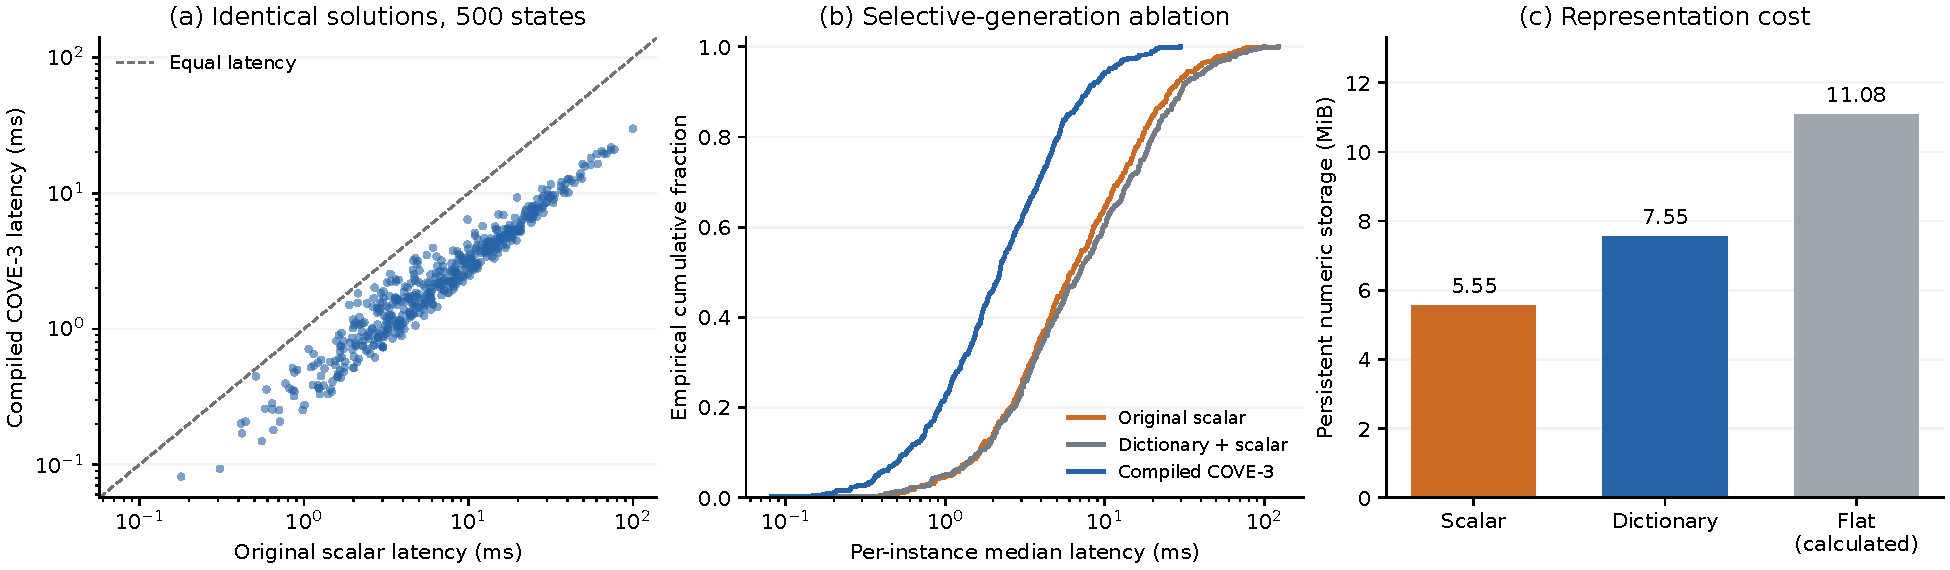
\includegraphics[width=\textwidth]{figures/contour-ablation.pdf}
\caption{Primary matched-output experiment. (a) Each point is one state's median of five timings. (b) Empirical latency distributions for all three configurations. (c) Persistent typed-array storage; the flat footprint is calculated. Outputs and logical counts are identical across configurations.}
\label{fig:contour-ablation}
\end{figure*}

\hypertarget{attribution-storage-and-initialization}{%
\subsection{Attribution, storage, and initialization}\label{attribution-storage-and-initialization}}

The dictionary-plus-scalar ablation is slower than the frozen original:
7.00 versus 6.19 ms median. Dictionary indirection and bookkeeping alone
therefore do not explain the gain. Enabling selective generation reduces
its median to 2.20 ms. This controlled ablation supports attribution to
avoiding rejected child construction and its associated call/path
overhead. It does not isolate each micro-operation within that
generator.

\textbf{Budget-policy negative control.} On evaluation state 0, setting
the global cap to 50,375 visits makes both the original and
budget-preserving implementations report exhaustion. A control that
deletes only the batched charges returns a 24-turn solution at that cap,
having changed what counts as work. The original reference completes a
different 23-turn sequence after 303,683 logical visits under the
default allowance. This constructive witness motivates preserving the
capped policy; it is not a frequency estimate or a claim that the
uncharged generator is invalid under its own different budget
definition. The state, outputs, source hashes, and control
transformation are archived in
\href{https://github.com/nahin333/rubikscube/blob/main/research/results/budget-witness.json}{budget-witness.json}.

\begin{table}[H]
\caption{Persistent numeric storage. The flat footprint is calculated, not a measured flat-solver latency or peak heap.}
\centering\small
\begin{tabularx}{\columnwidth}{@{}Lrr@{}}
\toprule
Representation & Bytes & MiB \\
\midrule
Scalar byte distances & 5,815,245 & 5.55 \\
Dictionary contours & 7,913,041 & 7.55 \\
Flat 32-bit contours, calculated & 11,621,325 & 11.08 \\
\bottomrule
\end{tabularx}
\end{table}

Full standalone construction takes 604.7 ms for the scalar baseline and
815.5 ms for compiled tables in the single recorded setup observation.
Compilation therefore has a real upfront cost. The browser posts its
first scalar solution before compiling in the worker; later requests use
the compiled tables. This scheduling avoids requiring full compilation
before the first response, but a request made during background
compilation can still wait. Worker termination remains the cancellation
mechanism. Neither lower peak heap nor faster cold end-to-end solving
has been established.

\hypertarget{external-cubejs-comparison}{%
\subsection{External cubejs comparison}\label{external-cubejs-comparison}}

\begin{table}[H]
\caption{Separate cubejs comparison on 200 shared scrambles. One timing per state; solution-quality targets differ.}
\centering\small
\begin{tabularx}{\columnwidth}{@{}Lrr@{}}
\toprule
Metric & cubejs 1.3.2 & Compiled COVE-3 \\
\midrule
Verified states & 200/200 & 200/200 \\
Median latency, ms ↓ & 42.932 & \textbf{3.916} \\
P95 latency, ms ↓ & 246.646 & \textbf{14.319} \\
Mean moves ↓ & \textbf{21.71} & 22.77 \\
Maximum moves ↓ & \textbf{22} & 26 \\
\bottomrule
\end{tabularx}
\end{table}

The external comparison confirms a useful application latency/length
tradeoff, while the primary experiment establishes an additional
improvement at identical output quality relative to our previous solver.
The new contour optimization is not credited with inventing the baseline
two-phase decomposition or with proving lower asymptotic complexity than
cubejs.

\begin{figure*}[t]
\centering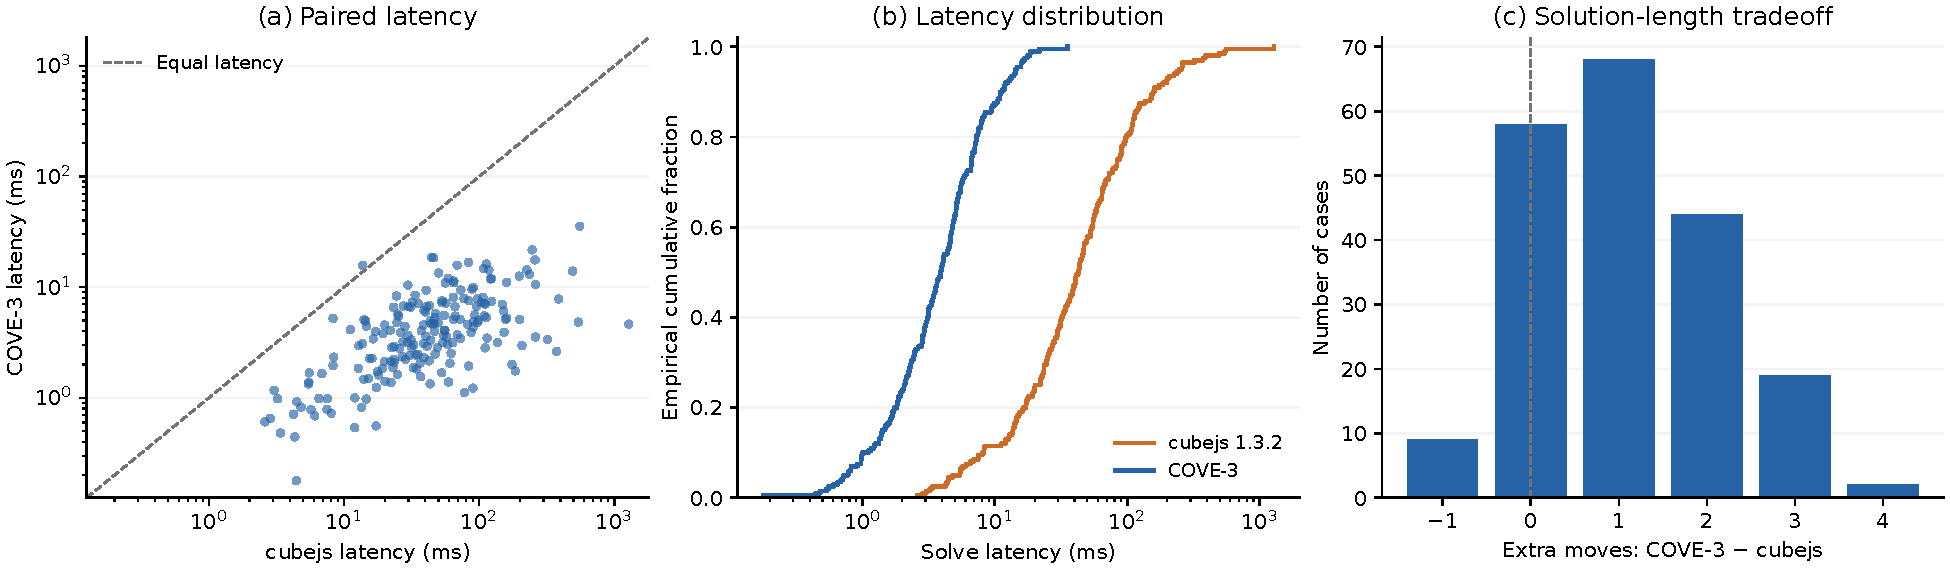
\includegraphics[width=\textwidth]{figures/solver-comparison.pdf}
\caption{Separate external cubejs comparison: paired latency, latency distributions, and extra moves. Different length targets prevent an equal-quality speedup claim.}
\label{fig:solver-comparison}
\end{figure*}

\hypertarget{correctness-and-application-behavior}{%
\subsection{Correctness and application behavior}\label{correctness-and-application-behavior}}

\begin{table*}[t]
\caption{Verification evidence. Counts concern different checks and should not be pooled as independent samples.}
\centering\small
\begin{tabularx}{\textwidth}{@{}p{0.23\textwidth}Lp{0.22\textwidth}@{}}
\toprule
Check & Coverage & Outcome \\
\midrule
Compiled successor certificates & All 19,353,600 abstract transitions; both masks and distance values & Matched scalar tests \\
Trace equivalence fixtures & 139 solved, single-turn, and separate legal-state cases & Identical moves, splits, and logical counts \\
Global-cap boundaries & 15 limits, including checkpoint and success/failure boundaries & Matching count-based outcomes and progress \\
Primary benchmark & 500 states × 3 configurations × 5 repetitions & All identical outputs; all sticker replays passed \\
Existing practical regression & 219 cases; 1000 cubie/sticker transitions; 40,320 permutation ranks & Passed \\
Existing exact-search regression & 2013 searches against shallow independent BFS and cross-checks & Passed \\
Browser integration & Initial scalar response, compiled follow-up, desktop/mobile viewport,
playback, photos, cancellation, worker failure & Passed locally and deployed \\
\bottomrule
\end{tabularx}
\end{table*}

The tests support the implementation but do not constitute a complete
formal verification of JavaScript, geometric transitions, or visual
recognition. The photo examples test input handling and symbolic
solving, rather than unconstrained real-world perception accuracy.

The application also retains earlier exact-search storage improvements.
On the archived ten-turn instance, bidirectional BFS stores 775,168
entries instead of 1,243,298 while preserving the optimal length. Those
changes are a separate implementation result, not an effect of contour
compilation; their fixed-instance measurements remain in
\href{https://github.com/nahin333/rubikscube/blob/main/research/results/exact-search.json}{exact-search.json}.

\hypertarget{follow-up-extensions-preserved-behavior-without-a-speedup}{%
\subsection{Follow-up extensions: preserved behavior without a speedup}\label{follow-up-extensions-preserved-behavior-without-a-speedup}}

The two research variants in Sections 4.6--4.7 were developed on a
100-state pilot (seed \texttt{0xb217ef}), then fixed before a separate
500-state evaluation (seed \texttt{0x83d92a}). Each has its own
interleaved contour-baseline run with five repetitions, 20 warmup states
(seed \texttt{0xabc123}), alternating order and corpus direction, and
independent sticker replay. Cache allocation is included in solve
latency; shared table construction is excluded. This is a single-machine
follow-up, not a preregistered or cross-device study. All 500 states,
repeated timings, outputs, and source hashes are archived separately for
\href{https://github.com/nahin333/rubikscube/blob/main/research/results/failure-replay.json}{failure
replay} and
\href{https://github.com/nahin333/rubikscube/blob/main/research/results/corridor-traversal.json}{chain
traversal}.

\begin{table*}[t]
\caption{Follow-up negative results on 500 separate states, five repetitions. Each candidate has its own contemporaneous contour baseline; medians are not pooled across runs.}
\centering\small
\begin{tabularx}{\textwidth}{@{}Lrrr@{}}
\toprule
Extension & Baseline median, ms & Candidate median, ms & Faster states \\
\midrule
Exact-cost failure replay & \textbf{2.123} & 2.507 & 41/500 \\
Deferred-charge chain traversal & \textbf{1.954} & 2.683 & 25/500 \\
\bottomrule
\end{tabularx}
\end{table*}

Failure replay records 966,438 cache hits and replaces 13,460,309
logical visits per single traversal of the corpus. Actual generated
visits fall from 26,899,938 to 25,852,443, a 3.89\% reduction: many
logically replayed visits were already skipped by contour masks. The
median of paired baseline/candidate speed ratios is 0.839, indicating
slowdown, despite the reduced generated work. Its additional 0.75 MiB
cache and lookup overhead do not pay off in this implementation.

Chain traversal removes 4,053,590 recursive calls while processing
exactly the same 26,899,938 generated visits. Its paired median speed
ratio is 0.683. Debt bookkeeping and the changed traversal structure
fail to improve measured latency. These results identify a limit of
call-count-based optimization: reducing recursion or generated visits
alone does not establish an execution-time gain. We have not profiled
individual micro-operations, so the data do not isolate the cause of
each slowdown.

\begin{figure*}[t]
\centering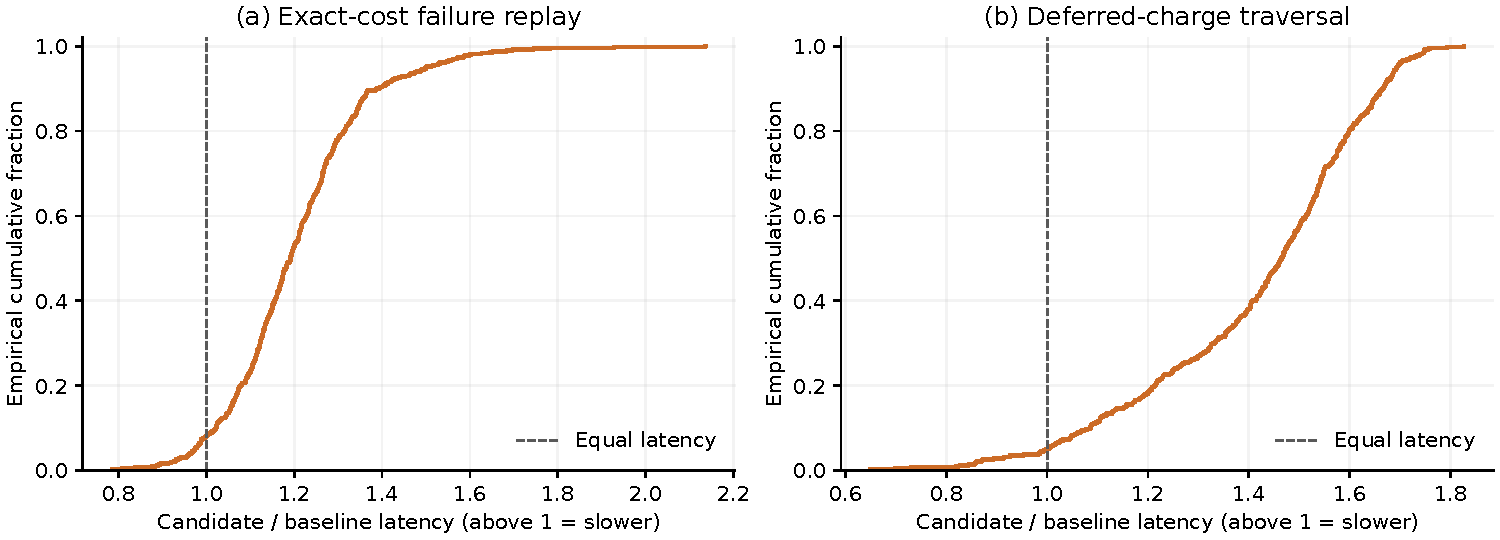
\includegraphics[width=\textwidth]{figures/research-extensions.pdf}
\caption{Follow-up experiments: per-instance latency ratios relative to the concurrently interleaved contour baseline. Ratios above one indicate slower execution. Both transformations preserve the tested count-based contract, but neither improves corpus median latency.}
\label{fig:research-extensions}
\end{figure*}

Separate correctness tests cover 169 solved, single-turn, and
legal-state fixtures for both variants. Fifteen global caps test both
variants and a deliberately collision-heavy two-slot replay cache,
checking exact outputs, counts, and progress notifications. Zero-timeout
guards also remain enforced. Both variants preserve every tested output
and count contract, but neither is enabled in the application. These are
correctness constructions and negative empirical findings, not
additional demonstrated speedups or certified first-ever algorithms.

\hypertarget{limitations}{%
\section{Limitations}\label{limitations}}

\textbf{Novelty boundary.} Two-phase search, pattern databases,
selective generation, bit masks, and dictionary coding have prior
foundations. This work contributes a particular compiled representation
and count-budget-preserving implementation with controlled evidence. The
literature review does not establish a new general search paradigm, a
first-ever use of the combination, or state-of-the-art solving
performance.

\textbf{Follow-up scope.} The failure-replay proposition assumes the
complete subtree key includes every path-dependent restriction. Adding
ancestor-cycle pruning or other history-dependent rules requires a new
argument. The research variants are prototypes evaluated in Node; they
are not enabled in the browser, and their measured slowdowns do not
prove that every implementation of these ideas must be slower.

\textbf{Resource tradeoffs.} Compiled tables use 36.07\% more persistent
numeric storage than scalar distances and add preprocessing. Temporary
BFS queues, compiler maps, garbage collection, and peak browser heap are
unmeasured. Deferred compilation changes scheduling rather than
eliminating its cost.

\textbf{Search guarantees.} Compilation preserves the baseline's
count-based behavior, including its limitations. The practical solver
returns a first completion, applies finite resource caps, and can fail
on a valid cube. It is not globally optimal or complete under those
caps. Faster execution can change real timeout outcomes, so the
equivalence theorem excludes an intervening wall-clock guard.

\textbf{Evaluation coverage.} Measurements use one processor and
runtime, synthetic pseudorandom states, a finite corpus, and a
deterministic experiment order. Five repetitions and paired bootstrap
intervals do not establish cross-machine or cross-browser performance.
The corpus was reused during final verification; this is not an
independently held-out, preregistered study. A mobile-sized Chromium
viewport is not a physical-phone performance evaluation.

\textbf{Comparator coverage.} The primary scalar baseline isolates our
implementation change. The external cubejs baseline has a different
length target, and no optimized native solver, modern min2phase
implementation, or learned solver is evaluated. The flat compiled
storage calculation is not a flat-code runtime ablation.

\textbf{Scope.} Compiled solving supports the fixed 3×3 model. The
application's exact demonstrations also support 2×2, but arbitrary-size
center solving, edge reduction, inner-layer moves, and parity repair for
larger cubes are not implemented. There is no learned model or evaluated
autonomous vision contribution.

\hypertarget{conclusion}{%
\section{Conclusion}\label{conclusion}}

Budget-preserving contour compilation improves COVE-3 by generating only
phase-2 children that pass its established abstract bounds. Dictionary
encoding reduces storage relative to flat signatures, and batched
charges preserve the scalar solver's logical limits and deterministic
output selection. On 500 states, median latency falls from 6.19 to 2.20
ms with identical solutions and 79.33\% fewer recursive calls. The cost
is an increase from 5.55 to 7.55 MiB of persistent tables and additional
compilation work. This establishes an improvement over our previous
solver at matched output quality. The accounting argument also supports
exact-cost failure replay and deferred sibling charges, but both tested
extensions are slower than the compiled baseline. Their negative results
reinforce the need for measured latency, not just smaller work counters.
Future evaluation should cover mobile hardware, alternative
representations, and newer solvers at matched targets.

\bibliographystyle{ieeenat_fullname}
\bibliography{references}
\end{document}
